% !TEX TS-program = xelatex
% !BIB program = bibtex
% !TeX spellcheck = ru_RU
% !TEX root = talk.tex

\documentclass
  [ russian
  , aspectratio=1610 % Для защит онлайн лучше использовать разрешение не 4х3
  ] {beamer}


% !TeX spellcheck = ru_RU
% !TEX root = vkr.tex
% Опциональные добавления используемых пакетов. Вполне может быть, что они вам не понадобятся, но в шаблоне приведены примеры их использования.
\usepackage{tikz} % Мощный пакет для создание рисунков, однако может очень сильно замедлять компиляцию
\usetikzlibrary{decorations.pathreplacing,calc,shapes,positioning,tikzmark}

% Библиотека для TikZ, которая генерирует отдельные файлы для каждого рисунка
% Позволяет ускорить компиляцию, однако имеет свои ограничения
% Например, ломает пример выделения кода в листинге из шаблона
% \usetikzlibrary{external}
% \tikzexternalize[prefix=figures/]

\newcounter{tmkcount}

\tikzset{
    use tikzmark/.style={
            remember picture,
            overlay,
            execute at end picture={
                    \stepcounter{tmkcount}
                },
        },
    tikzmark suffix={-\thetmkcount}
}

\usepackage{booktabs} % Пакет для верстки "более книжных" таблиц, вполне годится для оформления результатов
% В шаблоне есть команда \multirowcell, которой нужен этот пакет.
\usepackage{multirow}
\usepackage{siunitx} % для таблиц с единицами измерений

% Для названий стоит использовать \textsc{}
\newcommand{\OCaml}{\textsc{OCaml}}
\newcommand{\miniKanren}{\textsc{miniKanren}}
\newcommand{\BibTeX}{\textsc{BibTeX}}
\newcommand{\vsharp}{\textsc{V$\sharp$}}
\newcommand{\fsharp}{\textsc{F$\sharp$}}
\newcommand{\csharp}{\textsc{C\#}}
\newcommand{\GitHub}{\textsc{GitHub}}
\newcommand{\SMT}{\textsc{SMT}}



\usepackage{makecell}

\newcommand{\gdrive}{\textsc{Google Drive}}
\newcommand{\bukyvedefont}{Buky Vede}
\newcommand{\flavuniversalfont}{Flavius Universal}
\newcommand{\ponomarunicodefont}{Ponomar Unicode}
\newcommand{\menaionunicodefont}{Menaion Unicode}
\newcommand{\unicode}{Unicode}
\newcommand{\win}{Windows-1251}


\newcommand{\json}{\textsc{JSON}}
\newcommand{\postgresql}{\textsc{PostgreSQL}}
\newcommand{\sql}{\textsc{SQL}}
\newcommand{\api}{\textsc{API}}

\newcommand{\overleaf}{\textsc{Overleaf}}
\newcommand{\vscode}{\textsc{VS Code}}
\newcommand{\python}{\textsc{Python}}
\newcommand{\vuejs}{\textsc{Vue.js}}
\newcommand{\django}{\textsc{Django}}
\newcommand{\pytest}{\textsc{pytest}}
\newcommand{\ruff}{\textsc{ruff}}
\newcommand{\docker}{\textsc{Docker}}
\newcommand{\makefile}{\textsc{Makefile}}
\newcommand{\make}{\textsc{GNU Make}}
\newcommand{\word}{\textsc{Microsoft Word}}
\newcommand{\librewriter}{\textsc{Libre Office Writer}}
\newcommand{\docx}{\textsc{docx}}
\newcommand{\pypdf}{\textsc{PyPDF2}}
\newcommand{\xelatex}{\textsc{XeLaTeX}}
\newcommand{\nginx}{\textsc{nginx}}
\newcommand{\sus}{\textsc{SUS}}
\newcommand{\systemusabilityscale}{\textsc{System Usability Scale}}
\newcommand{\gunicorn}{\textsc{gunicorn}}
\newcommand{\pdf}{\textsc{PDF}}
\newcommand{\tex}{\textsc{TeX}}



\newcommand{\todo}[1]{\textcolor{red}{TODOP: #1}}
\newcommand{\todov}[1]{\textcolor{orange}{TODOV: #1}}





\definecolor{cellgreen}{RGB}{198, 239, 206}
\definecolor{cellorange}{RGB}{255, 229, 153}
\definecolor{cellred}{RGB}{255, 199, 206}


\definecolor{eclipseGreen}{RGB}{63,127,95}
% \lstdefinelanguage{ocaml}{
% keywords={@type, function, fun, let, in, match, with, when, class, type,
% nonrec, object, method, of, rec, repeat, until, while, not, do, done, as, val, inherit, and,
% new, module, sig, deriving, datatype, struct, if, then, else, open, private, virtual, include, success, failure,
% lazy, assert, true, false, end},
% sensitive=true,
% commentstyle=\small\itshape\ttfamily,
% keywordstyle=\ttfamily\bfseries, %\underbar,
% identifierstyle=\ttfamily,
% basewidth={0.5em,0.5em},
% columns=fixed,
% fontadjust=true,
% literate={->}{{$\to$}}3 {===}{{$\equiv$}}1 {=/=}{{$\not\equiv$}}1 {|>}{{$\triangleright$}}3 {\\/}{{$\vee$}}2 {/\\}{{$\wedge$}}2 {>=}{{$\ge$}}1 {<=}{{$\le$}} 1,
% morecomment=[s]{(*}{*)}
% }

\makeatletter
\@ifclassloaded{beamer}{
    %%% Обязательные пакеты
    %% Beamer
    \usepackage{beamerthemesplit}
    \usetheme{SPbGU}
    \beamertemplatenavigationsymbolsempty
    \usepackage{appendixnumberbeamer}

    %% Локализация
    \usepackage{fontspec}
    \setmainfont{CMU Serif}
    \setsansfont{CMU Sans Serif}
    \setmonofont{CMU Typewriter Text}

    %\setmonofont{Fira Code}[Contextuals=Alternate,Scale=0.9]
    %\setmonofont{Inconsolata}
    \usepackage{polyglossia}
    \setmainlanguage{russian}
    \setotherlanguage{english}

    %% Графика
    \usepackage{pdfpages} % Позволяет вставлять многостраничные pdf документы в текст

    % Математические окружения с русским названием
    \newtheorem{rutheorem}{Теорема}
    \newtheorem{ruproof}{Доказательство}
    \newtheorem{rudefinition}{Определение}
    \newtheorem{rulemma}{Лемма}
    \usepackage{fancyvrb}
}
{}
\makeatother

\usepackage[autostyle]{csquotes} % Правильные кавычки в зависимости от языка
\usepackage{totcount}
\usepackage{setspace}
\usepackage{amsmath, amsfonts, amssymb, amsthm, mathtools} % "Адекватная" работа с математикой в LaTeX

\usepackage{fontspec}
\newfontfamily{\bukyvede}[
  Path = fonts/
]{bukyvede.ttf}

\newfontfamily{\flaviusuniversal}[
  Path = fonts/
]{FlaviusUniversal.ttf}

\newfontfamily{\ponomarunicode}[
  Path = fonts/
]{PonomarUnicode.otf}

\newfontfamily{\menaionunicode}[
  Path = fonts/
]{menaionunicode.otf}

\makeatletter

\input{pretitle.tex}
\input{title.tex}

\newcommand{\academicGroup}{\my@title@group@ru}
\newcommand{\advisorChair}{\my@title@chair@ru}
% То, что в квадратных скобках, отображается внизу по центру каждого слайда.
\title[Редактор кириллических текстов]{\my@title@title@ru}
% То, что в квадратных скобках, отображается в левом нижнем углу.
\author[\my@title@author@ru]{\my@title@author@ru}
\institute[СПбГУ]{}
\date[08 июня 2026 г.]{}
\newcommand{\supervisor}{\my@title@supervisor@ru}
\newcommand{\supervisorPosition}{\my@title@supervisorPosition@ru}
\newcommand{\consultant}{\my@title@consultant@ru}
\newcommand{\consultantPosition}{\my@title@consultantPosition@ru}
\newcommand{\reviewer}{\my@title@reviewer@ru}
\newcommand{\reviewerPosition}{\my@title@reviewerPosition@ru}
\newcommand{\defenseYear}{\my@title@year@ru}

\makeatother
\begin{document}
{
\setbeamertemplate{footline}{}
% Лого университета или организации, отображается в шапке титульного листа
\begin{frame}
    
\includegraphics[width=1.4cm]{figures/SPbGU_Logo.png}
    \vspace{-35pt}
    \hspace{-10pt}
    \begin{center}
        \begin{tabular}{c}
            \scriptsize{Санкт-Петербургский государственный университет} \\
            \scriptsize{\advisorChair}
        \end{tabular}
        \titlepage
    \end{center}

    \btVFill

    {\scriptsize
        % % У научного руководителя должна быть указана научная степень
        \textbf{Научный руководитель:}  \supervisorPosition~\supervisor \\
        % % Консультанта может и не быть. Должна быть указана должность или ученая степень
        % \textbf{Консультант:}  \consultantPosition~\consultant \\
        % % Для учебной практики не обязателен. Должна быть указана должность или ученая степень
        \textbf{Рецензент:} \reviewerPosition~\reviewer \\
    }
    \makeatother
    \begin{center}
        \vspace{5pt}
        \scriptsize{Санкт-Петербург\\ \defenseYear}
    \end{center}
\end{frame}
}

\begin{frame}{Введение}
    \begin{itemize}
        \item Оцифровка кириллических рукописей: \textbf{\enquote{Цифровой летописец}} совместно с научно-исследовательским отделом \textbf{рукописей Библиотеки Российской академии наук}
        \item Сотрудники сталкиваются с проблемами при подготовке текстов для публикации:
        \begin{enumerate}
            \item \textbf{Неконсистентность отображения} при смене шрифта
            \begin{center}
                
\includegraphics[width=0.4\textwidth]{figures/flavexp-bad-conversion.png}
            \end{center}
            \item Неудобство набора \textbf{специфичных кириллических символов}
        \end{enumerate}
        \item Процесс подготовки текста к публикации усложняется
        \item Необходим удобный инструмент, обеспечивающий корректную работу с кириллическими шрифтами
    \end{itemize}
\end{frame}

\begin{frame}
    \frametitle{Существующие решения}

    \begin{itemize}
        \item \textbf{Microsoft Word}
        \begin{itemize}
            \item Де-факто стандарт
            \item Доступен экспорт в PDF
            \item Недостатки:
            \begin{enumerate}
                \item \textbf{Нет поддержки конвертации} кириллических шрифтов: при \textbf{смене шрифта} текст может \enquote{сломаться}
                \item Нет встроенного инструмента для \textbf{набора спецсимволов}
            \end{enumerate}
        \end{itemize}
        \item \textbf{Overleaf}
        \begin{itemize}
            \item Экспорт в PDF
            \item Использование TeX
            \item Недостатки:
            \begin{enumerate}
                \item \textbf{Компиляция лимитирована} по объёму (при превышении лимита~--- платно)
                \item \textbf{Нет поддержки конвертации} кириллических шрифтов
                \item Нет встроенного инструмента для \textbf{набора спецсимволов}
                \item \enquote{Неблизко} экспертам по рукописям
            \end{enumerate}
        \end{itemize}
    \end{itemize}
\end{frame}

\begin{frame}
    \frametitle{Выводы}

    \begin{itemize}
        \item \textbf{Нет инструмента} для работы с кириллическими и церковнославянскими текстами

        \vspace{1em}

        \item Основные недостатки существующих решений:
        \begin{enumerate}
            \item \textbf{Неудобный набор} специфичных кириллических символов
            \item Не учитываются особенности шрифтов, отсутствует механизм \textbf{корректной конвертации}
            \item \textbf{Ограничения по объему} текста в бесплатных версиях
        \end{enumerate}
    \end{itemize}
\end{frame}

% % Обязательный слайд: четкая формулировка цели данной работы и постановка задачи
% % Описание выносимых на защиту результатов, процесса или особенностей их достижения и т.д.
\begin{frame}{Постановка задачи}
    \textbf{Целью} работы является создание приложения для работы с оцифрованными кириллическими рукописями.
    \vspace{1em}

    \textbf{Задачи:}
    \begin{enumerate}
        \item Собрать и проработать требования к инструменту
        \item Провести сравнительный обзор шрифтов, используемых при наборе кириллических текстов
        \item Спроектировать архитектуру приложения
        \item Реализовать разработанное решение
        \item Развернуть приложение на сервере
        \item Обеспечить тестовое покрытие кода backend API приложения не менее 70\% операторов (statements)
        \item Провести апробацию инструмента среди пользователей
    \end{enumerate}
\end{frame}

% %Идеально, если есть по одному слайду на каждую поставленную задачу

\begin{frame}{Требования}
    \textbf{Функциональные требования:}
    \begin{enumerate}
        \item \textbf{Импорт} и \textbf{экспорт} файлов в форматах \textbf{PDF}, \textbf{DOCX}, \textbf{TXT}
        \item Генерация \textbf{PDF} с использованием \textbf{XeLaTeX}
        \item \textbf{Корректная конвертация} текста между шрифтами
        \item Конвертация между кириллицей и \textbf{глаголицей}
        \item Встроенная \textbf{экранная клавиатура} для ввода спецсимволов
        \item Возможность добавления \textbf{пользовательских шрифтов}
    \end{enumerate}

    \vspace{1em}

    \textbf{Нефункциональные требования:}
    \begin{enumerate}
        \item Кроссплатформенность
        \item Интуитивно понятный интерфейс
    \end{enumerate}
\end{frame}

\begin{frame}{Обзор шрифтов}

    Рассматривалось 5 шрифтов:
    \begin{itemize}
        \item BukyVede
        \item Flavius Unicode Universal (и FlavExp Unicode Universal)
        \item Menaion Unicode
        \item Ponomar Unicode
    \end{itemize}

    Сравнение проводилось по 5 выделенным категориям:
    \begin{enumerate}
        \item Церковнославянский алфавит
        \item Дополнительные буквы из старославянского языка
        \item Выносные буквы (буквотитла)
        \item Диакритические знаки
        \item Знаки препинания
    \end{enumerate}

    \begin{center}
    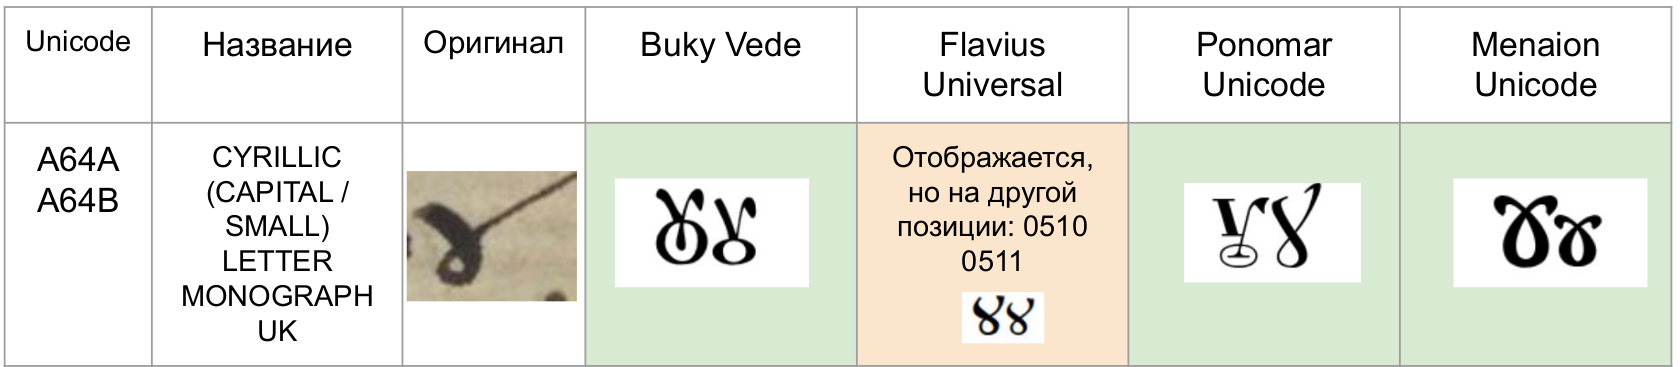
\includegraphics[width=0.8\textwidth]{figures/compare_monograph_uk.png}
    \end{center}
\end{frame}


\begin{frame}{Обзор шрифтов}

    \begin{table}[H]
            \caption{Итоги сравнения, количество поддерживаемых символов}
            \label{tab:results}
            \centering
            \begin{tabular}{|c|c|c|c|c|c|}
                \hline
                          & Buky & \textbf{Flavius} & Ponomar & \textbf{Menaion} & Всего в\\
                Категория & Vede & \textbf{Universal} & Unicode & \textbf{Unicode} & категории \\
                \hline
                1 & 86 & 82 & 86 & 86 & 86\\
                \hline
                2 & 45 & 28 & 42 & 54 & 54\\
                \hline
                3 & 32 & 0  & 29 & 31 & 32\\
                \hline
                4 & 24 & 15 & 24 & 25 & 26\\
                \hline
                5 & 6  & 6  & 6  & 6  & 6\\
                \hline
                \textbf{Итог} & 193 & \textbf{131} & 187 & \textbf{202} & 204\\
                \hline
            \end{tabular}
        \end{table}

     Выводы:
    \begin{itemize}
        \item \textbf{Menaion Unicode}~--- лучший по количеству корректно отображаемых символов
        \item Необходим инструмент конвертации между шрифтами, чтобы символы не \enquote{ломались}
     \end{itemize}
\end{frame}

\begin{frame}{Архитектура решения (backend)}

    Одностраничное веб-приложение (SPA)
    \vspace{1em}

    Используемые технологии:
    \begin{itemize}
        \item Фронтэнд: \textbf{Vue.js}
        \item Бэкэнд: Python (\textbf{FastAPI}) и библиотеки
        \begin{itemize}
            \item docx
            \item PyPDF
        \end{itemize}
        \item Сборка PDF: \textbf{XeLaTeX}~--- встроенная поддержка \textbf{Unicode}
        \item Инфраструктура:
        \begin{itemize}
            \item \textbf{nginx}
            \item \textbf{Docker}
            \item \textbf{make}
        \end{itemize}
    \end{itemize}
    % \item В реализации интересны архитектура, библиотеки, инструменты
%     \item Не надо добавлять на слайд примеры кода
\end{frame}

\begin{frame}{Архитектура решения: процесс работы с PDF}

    \begin{center}
        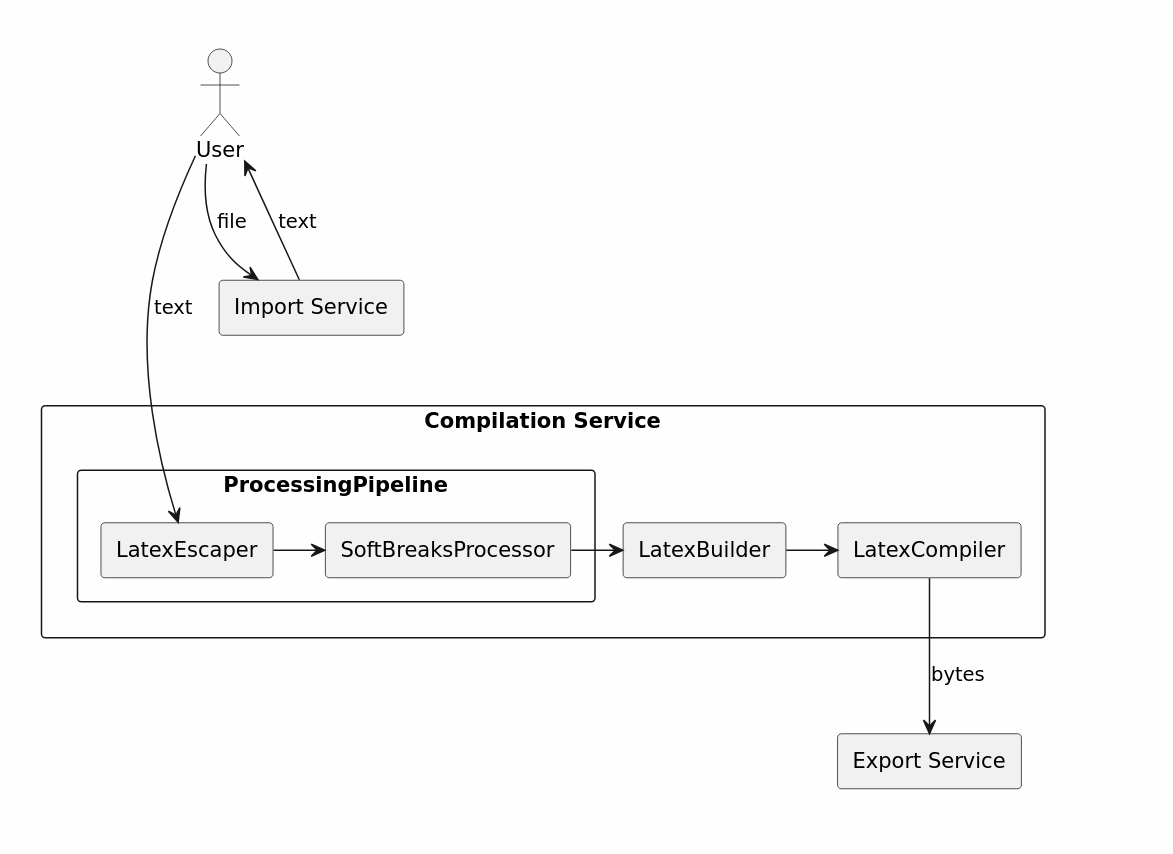
\includegraphics[width=0.6\textwidth]{figures/services-flow-new.png}
    \end{center}
\end{frame}

\begin{frame}{Реализация: внешний вид приложения}
    \begin{center}
        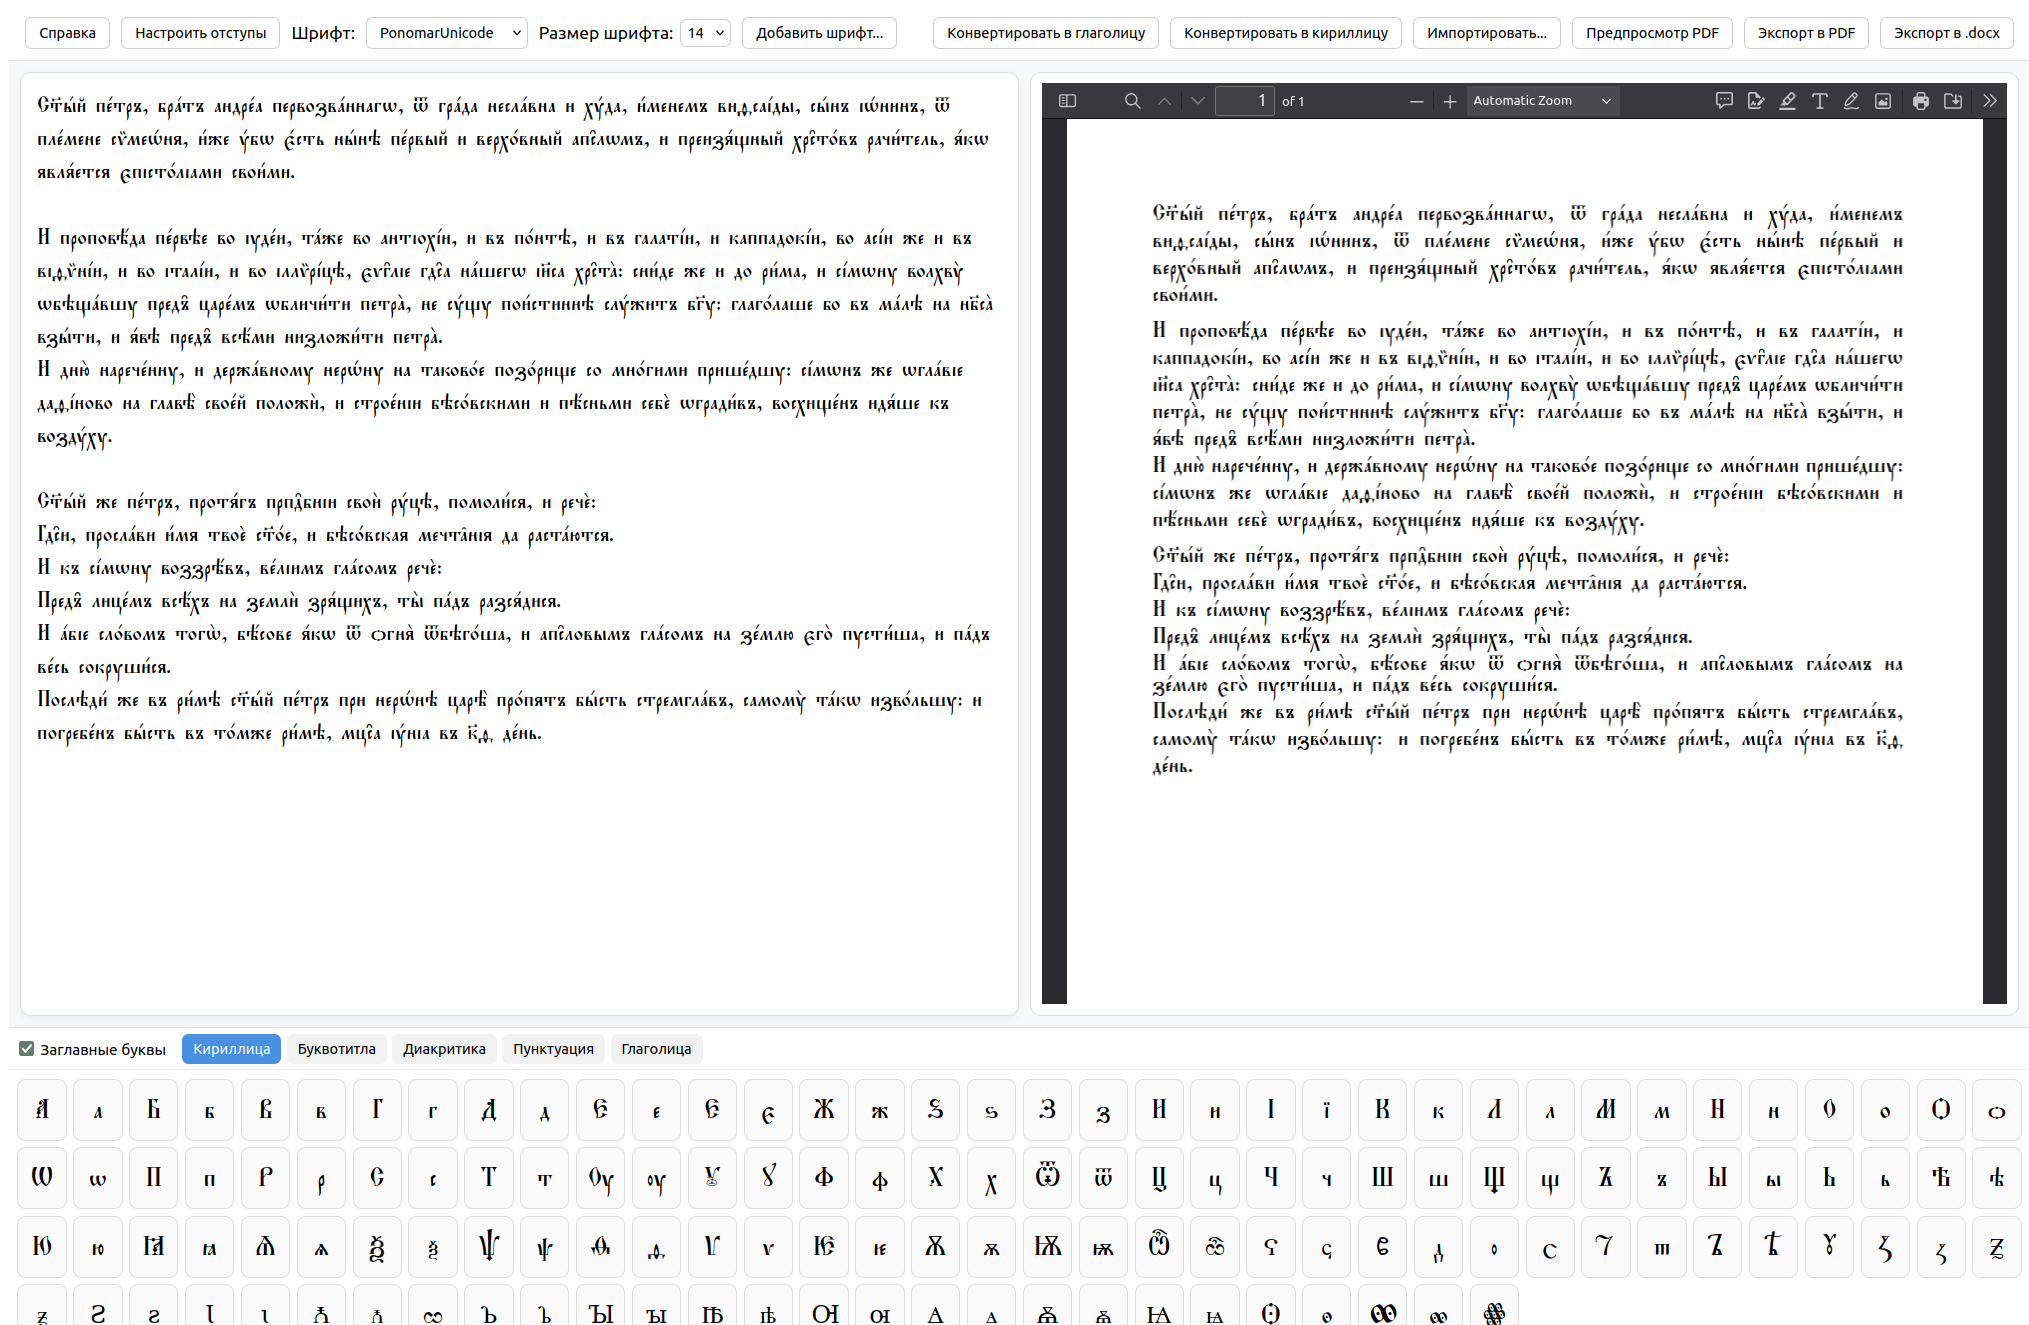
\includegraphics[width=0.8\textwidth]{figures/demo_new.png}
    \end{center}
\end{frame}

\begin{frame}{Развертывание}

    \begin{columns}

        \begin{column}{0.6\textwidth}
            \begin{itemize}
                \item Dockerfile:
                \begin{enumerate}
                    \item frontend
                    \item backend
                \end{enumerate}
                \item Docker Compose
                \item make deploy
            \end{itemize}
        \end{column}

        \begin{column}{0.4\textwidth}
            Развернутое веб-приложение:
            \begin{center}
                
\includegraphics[width=0.4\textwidth]{figures/qr-site.png}
            \end{center}
        \end{column}

    \end{columns}

\end{frame}

\begin{frame}{Апробация и тестирование}
    Апробация по методике SUS:
    \begin{itemize}
        \item 11 респондентов
        \item Итоговый балл: 73.9
    \end{itemize}

    \vspace{1em}

    Покрытие кода тестами (pytest): 89\% операторов
    \begin{center}
        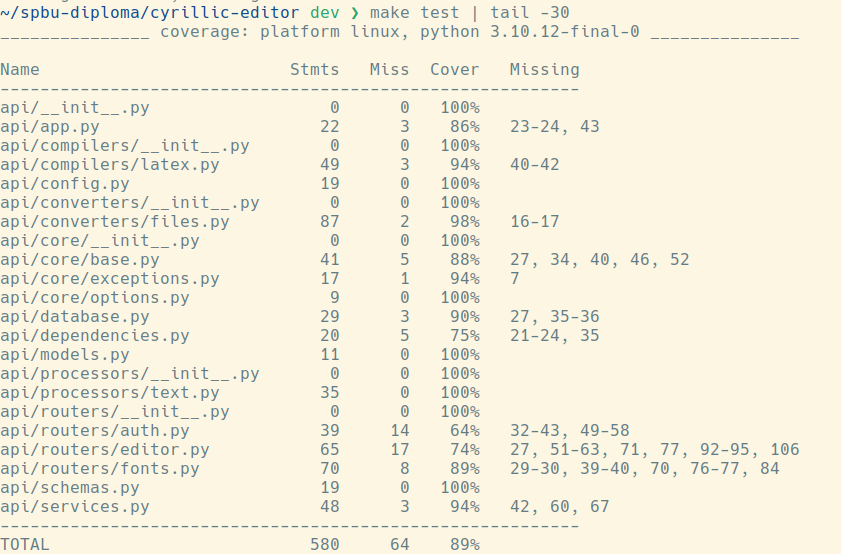
\includegraphics[width=0.5\textwidth]{figures/test_coverage.png}
    \end{center}
\end{frame}

\begin{frame}
    \frametitle{Результаты}
    В результате работы были выполнены следующие задачи:
    \begin{enumerate}
        \item Собраны и проработаны требования к инструменту
        \item Проведен сравнительный обзор кириллических шрифтов
        \begin{itemize}
            \item Определен лучший по количеству корректно отображаемых символов шрифт~--- Menaion Unicode
            \item Выявлены особенности отображения символов в различных шрифтах и разработан механизм их корректного сопоставления при конвертации
        \end{itemize}
        \item Спроектировано решение на основе требований
        \item Реализовано спроектированное решение
        \item Развернуто реализованное решение на сервере
        \item Проведена апробация среди пользователей, SUS: 73.9
        \item Обеспечено тестовое покрытие кода backend API приложения~--- 89\% операторов (statements)
    \end{enumerate}

    Код доступен по ссылке: \url{https://github.com/aleksandr-yavorovskiy/cyrillic-editor}

    % \begin{itemize}
    Результаты работы представлены на конференциях \enquote{IT-симпозиум~2026} и \enquote{СПИСОК~2026}.
    % \end{itemize}
\end{frame}

\appendix

\begin{frame}
    \frametitle{Дополнительный слайд}

    \begin{columns}
        \begin{column}{0.5\textwidth}
            Исходный код:
            \begin{center}
                
\includegraphics[width=0.4\textwidth]{figures/qr-github.png}
            \end{center}
        \end{column}

        \begin{column}{0.5\textwidth}
            Развернутое веб-приложение:
            \begin{center}
                
\includegraphics[width=0.4\textwidth]{figures/qr-site.png}
            \end{center}
        \end{column}

    \end{columns}
\end{frame}

\begin{frame}
    \frametitle{Дополнительный слайд}

    Смена шрифта: A => B

    FontToUnicode (A) => Unicode => UnicodeToFont (B)
    \begin{center}
        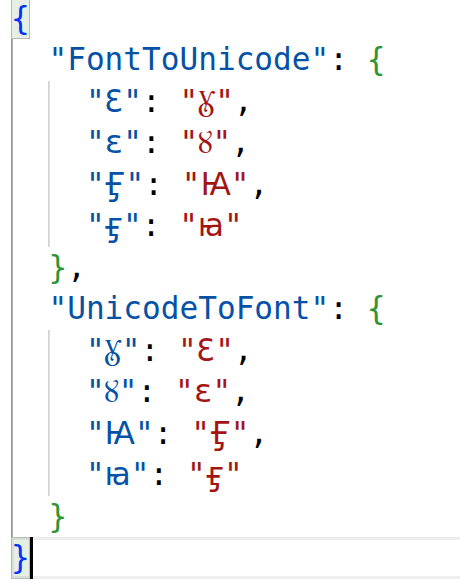
\includegraphics[width=0.3\textwidth]{figures/json_example.png}
    \end{center}
\end{frame}

\end{document}
